\chapter{Números quânticos e configurações eletrônicas}\label{ch:b1:quantum-numbers}

Encha um tubo de vidro com hidrogênio a baixa pressão, faça passar por
ele uma descarga elétrica e observe o brilho rosado através de um prisma.
A luz não se espalha em um arco-íris: ela se divide em quatro raias
nítidas --- uma vermelha, uma verde-azulada, duas violeta --- e nada
entre elas. Um sólido quente brilha em todos os comprimentos de onda; um
átomo de hidrogênio emite apenas um punhado deles. A explicação,
encontrada entre 1913 e 1926, é que a energia de um elétron em um átomo
não pode assumir qualquer valor: ela é \emph{quantizada}. Este capítulo
enuncia as regras dessa quantização tal como o químico as utiliza ---
quatro números quânticos, três regras de preenchimento --- e as
transforma na \omterm{def:b1:quantum-numbers:configuration}{configuração eletrônica} de cada átomo e de cada íon, a
chave da tabela periódica do próximo capítulo.

\begin{recall}
O Livro 1 (ano 10) distribuiu os elétrons dos vinte primeiros elementos
em camadas e \omterm{def:b1:quantum-numbers:orbital}{subcamadas}, 1s, 2s, 2p, 3s, 3p, e chamou de \omterm{def:b1:quantum-numbers:configuration}{elétrons de
valência} os elétrons da camada mais externa. Da física, usamos como
conhecido que a luz de comprimento de onda $\lambda$ é formada de fótons
de energia
$E = h\nu = hc/\lambda$, em que $h$ é a constante de Planck e $c$ a
velocidade da luz.
\end{recall}

\begin{omfigure}

\includegraphics[width=0.62\linewidth]{images/book2/ai/b1-01-street-lamps.jpg}

{\small Lâmpadas de sódio de baixa pressão na iluminação pública. A luz
delas é quase uma única raia amarelo-alaranjada: como o hidrogênio, um
átomo de sódio excitado só emite fótons de algumas energias precisas.}
\end{omfigure}

\section{Energias quantizadas: o espectro do hidrogênio}

\begin{definition}[Nível de energia, estado fundamental, estado excitado]\label{def:b1:quantum-numbers:energy-level}
A energia de um elétron ligado a um átomo só pode assumir certos
valores, os \emph{níveis de energia}\index{nivel de energia@nível de energia} do átomo. O zero de
energia é tomado quando o elétron está em repouso, infinitamente longe
do núcleo (o átomo está ionizado), de modo que todo nível de um elétron
ligado é negativo. O nível mais baixo é o \emph{estado fundamental}\index{estado fundamental};
todos os outros níveis são \emph{estados excitados}\index{estado excitado}.
\end{definition}

Um átomo passa de um \omterm{def:b1:quantum-numbers:energy-level}{nível de energia} $E_{\text{sup}}$ para um nível mais
baixo $E_{\text{inf}}$ emitindo um fóton, e do nível mais baixo para o
mais alto absorvendo um, de energia
\[
  h\nu = \frac{hc}{\lambda} = E_{\text{sup}} - E_{\text{inf}} .
\]
Um espectro de raias é, portanto, uma imagem das diferenças entre os
níveis.

\begin{theorem}[Níveis de energia do átomo de hidrogênio]\label{thm:b1:quantum-numbers:levels}
Os \omterm{def:b1:quantum-numbers:energy-level}{níveis de energia} do átomo de hidrogênio são
\[
  E_n = -\frac{E_R}{n^2}, \qquad n = 1, 2, 3, \dots,
  \qquad E_R = \qty{13.6}{eV},
\]
em que $E_R$ é a energia de Rydberg (corrigida pelo movimento do
núcleo). O \omterm{def:b1:quantum-numbers:energy-level}{estado fundamental} é $E_1 = \qty{-13.6}{eV}$ e a energia de
ionização do átomo é $E_R$.
% ledger: const:RyhcEV, ie:H (13.598 eV; levels computed in
% figdata/bachelor-1/hydrogen-levels.py)
\end{theorem}
\admitted

\begin{remark}[De onde vem a fórmula]\label{rem:b1:quantum-numbers:schrodinger}
A fórmula decorre da resolução da equação de Schrödinger do elétron no
campo do próton; essa resolução, e as formas das funções de onda que
ela fornece, são deduzidas no volume do 2.º ano. Niels Bohr havia
obtido os mesmos níveis em 1913 a partir de um modelo mais simples de
órbitas circulares, hoje abandonado.
\end{remark}

\begin{proposition}[A fórmula de Rydberg]\label{prop:b1:quantum-numbers:rydberg}
As raias emitidas pelo hidrogênio têm comprimentos de onda dados por
\[
  \frac{1}{\lambda} = R_H\left(\frac{1}{n_1^2} - \frac{1}{n_2^2}\right),
  \qquad n_2 > n_1 \ge 1, \qquad R_H = \frac{E_R}{hc},
\]
para a transição do nível $n_2$ para o nível $n_1$. As raias que
terminam no mesmo nível $n_1$ formam uma \emph{série}: Lyman para $n_1 = 1$
(ultravioleta), Balmer para $n_1 = 2$ (visível), Paschen para $n_1 = 3$
(infravermelho).
\end{proposition}

\begin{proof}
O fóton leva a energia perdida pelo átomo:
$hc/\lambda = E_{n_2} - E_{n_1} = -E_R/n_2^2 + E_R/n_1^2
= E_R\,(1/n_1^2 - 1/n_2^2)$. Dividindo por $hc$, obtém-se a fórmula.
\end{proof}

\begin{example}[A raia vermelha do hidrogênio]\label{ex:b1:quantum-numbers:halpha}
Para a transição $3 \to 2$: $\Delta E = 13.6\,(1/4 - 1/9) =
\qty{1.89}{eV}$. Com $hc = \qty{1240}{eV.nm}$ (a partir dos valores de $h$,
$c$ e $e$), $\lambda = 1240/1.89 = \qty{656}{nm}$: a raia vermelha.
As outras raias de Balmer, $4 \to 2$, $5 \to 2$, $6 \to 2$, caem em 486,
434 e \qty{410}{nm}; a seguinte, $7 \to 2$ em \qty{397}{nm}, já está
no ultravioleta. Os comprimentos de onda medidos, 656.3, 486.1, 434.0
e \qty{410.2}{nm}, concordam com precisão melhor que uma parte em dois
mil; a pequena diferença restante vem de medir no ar e não no vácuo.
% ledger: asd:Halpha, asd:Hbeta, asd:Hgamma, asd:Hdelta (computed values
% in figdata/out/bachelor-1-hydrogen-levels-balmer.dat)
\end{example}

\begin{omfigure}
\begin{tikzpicture}
\begin{axis}[
  width=0.62\linewidth, height=7.2cm,
  xmin=0, xmax=10, ymin=-14.5, ymax=0.6,
  axis x line=none, axis y line=left,
  ylabel={energia (eV)}, ytick={-14,-12,-10,-8,-6,-4,-2,0},
  tick label style={font=\small}, label style={font=\small},
  clip=false]
\pgfplotsinvokeforeach{-13.598,-3.400,-1.511,-0.850,-0.544}{
  \draw[black!70, line width=0.7pt] (axis cs:0.3,#1) -- (axis cs:9.6,#1);}
\draw[black!40, dashed] (axis cs:0.3,0) -- (axis cs:9.6,0);
\node[font=\small, anchor=west] at (axis cs:9.7,-13.598) {$n = 1$};
\node[font=\small, anchor=west] at (axis cs:9.7,-3.400) {$n = 2$};
\node[font=\small, anchor=west] at (axis cs:9.7,-1.511) {$n = 3$};
\node[font=\small, anchor=south west] at (axis cs:9.7,0.05) {$n \to \infty$};
% Lyman
\draw[-{Stealth}, violet!70!black, thick] (axis cs:1.0,-3.400) -- (axis cs:1.0,-13.598);
\draw[-{Stealth}, violet!70!black, thick] (axis cs:1.6,-1.511) -- (axis cs:1.6,-13.598);
\draw[-{Stealth}, violet!70!black, thick] (axis cs:2.2,-0.850) -- (axis cs:2.2,-13.598);
\node[font=\small, violet!70!black, anchor=west] at (axis cs:2.4,-9) {Lyman};
% Balmer
\draw[-{Stealth}, red!80!black, thick] (axis cs:4.4,-1.511) -- (axis cs:4.4,-3.400);
\draw[-{Stealth}, teal!80!black, thick] (axis cs:5.0,-0.850) -- (axis cs:5.0,-3.400);
\draw[-{Stealth}, blue!80!black, thick] (axis cs:5.6,-0.544) -- (axis cs:5.6,-3.400);
\node[font=\small, anchor=north] at (axis cs:5.0,-3.6) {Balmer};
% Paschen
\draw[-{Stealth}, black!60, thick] (axis cs:7.8,-0.850) -- (axis cs:7.8,-1.511);
\draw[-{Stealth}, black!60, thick] (axis cs:8.4,-0.544) -- (axis cs:8.4,-1.511);
\node[font=\small, anchor=north] at (axis cs:8.1,-1.7) {Paschen};
\end{axis}
\end{tikzpicture}

{\small Os \omterm{def:b1:quantum-numbers:energy-level}{níveis de energia} do hidrogênio, $E_n = -\qty{13.6}{eV}/n^2$,
desenhados em escala (calculados a partir da constante de Rydberg); os
níveis $n = 4,
5, \dots$ se acumulam logo abaixo de zero. Cada seta é um fóton
emitido; as setas que terminam no mesmo nível formam uma série.}
\end{omfigure}

\begin{omfigure}
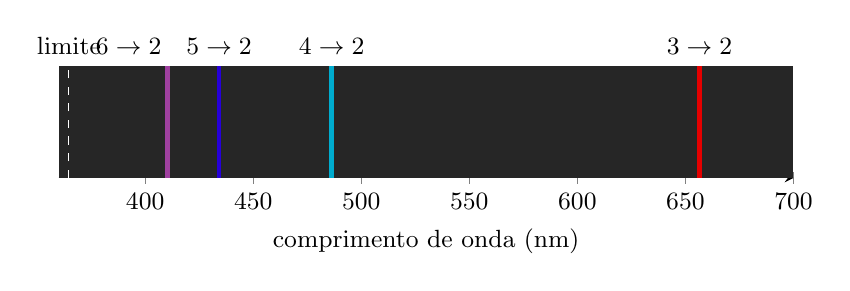
\begin{tikzpicture}
\begin{axis}[
  width=0.9\linewidth, height=3.0cm,
  xmin=360, xmax=700, ymin=0, ymax=1,
  axis x line=bottom, axis y line=none,
  xlabel={comprimento de onda (nm)}, xtick={400,450,500,550,600,650,700},
  tick label style={font=\small}, label style={font=\small},
  clip=false]
\fill[black!85] (axis cs:360,0) rectangle (axis cs:700,1);
% line positions: figdata/out/bachelor-1-hydrogen-levels-balmer.dat
\draw[line width=1.6pt, red!90!black] (axis cs:656.5,0) -- (axis cs:656.5,1);
\draw[line width=1.6pt, cyan!80!green] (axis cs:486.3,0) -- (axis cs:486.3,1);
\draw[line width=1.6pt, blue!70!violet] (axis cs:434.2,0) -- (axis cs:434.2,1);
\draw[line width=1.6pt, violet!75] (axis cs:410.3,0) -- (axis cs:410.3,1);
\draw[white, dashed] (axis cs:364.7,0) -- (axis cs:364.7,1);
\node[font=\small, anchor=south] at (axis cs:364.7,1.02) {limite};
\node[font=\small, anchor=south] at (axis cs:656.5,1.02) {$3\to2$};
\node[font=\small, anchor=south] at (axis cs:486.3,1.02) {$4\to2$};
\node[font=\small, anchor=south] at (axis cs:434.2,1.02) {$5\to2$};
\node[font=\small, anchor=south east] at (axis cs:412,1.02) {$6\to2$};
\end{axis}
\end{tikzpicture}

{\small As raias de Balmer calculadas pela fórmula de Rydberg
(comprimentos de onda no vácuo), sobre a faixa visível. Outras raias se
acumulam em direção ao limite da série, em \qty{364.7}{nm}, no ultravioleta.}
\end{omfigure}

\begin{history}[O átomo de Bohr, 1913]
Em 1913, Niels Bohr, um físico dinamarquês de 28 anos que trabalhava em
Manchester, propôs que o elétron do hidrogênio só podia girar em torno
do núcleo em certas órbitas, e que a luz era emitida quando ele saltava
de uma órbita para outra mais baixa. Seu modelo reproduzia exatamente as
raias de Balmer, e fornecia o valor da constante de Rydberg a partir de
$h$, $e$ e da massa do elétron. As órbitas não sobreviveram à mecânica
quântica de 1925--1926, mas os níveis quantizados sim. Bohr recebeu o
Prêmio Nobel de Física em 1922.
\end{history}

\begin{omfigure}
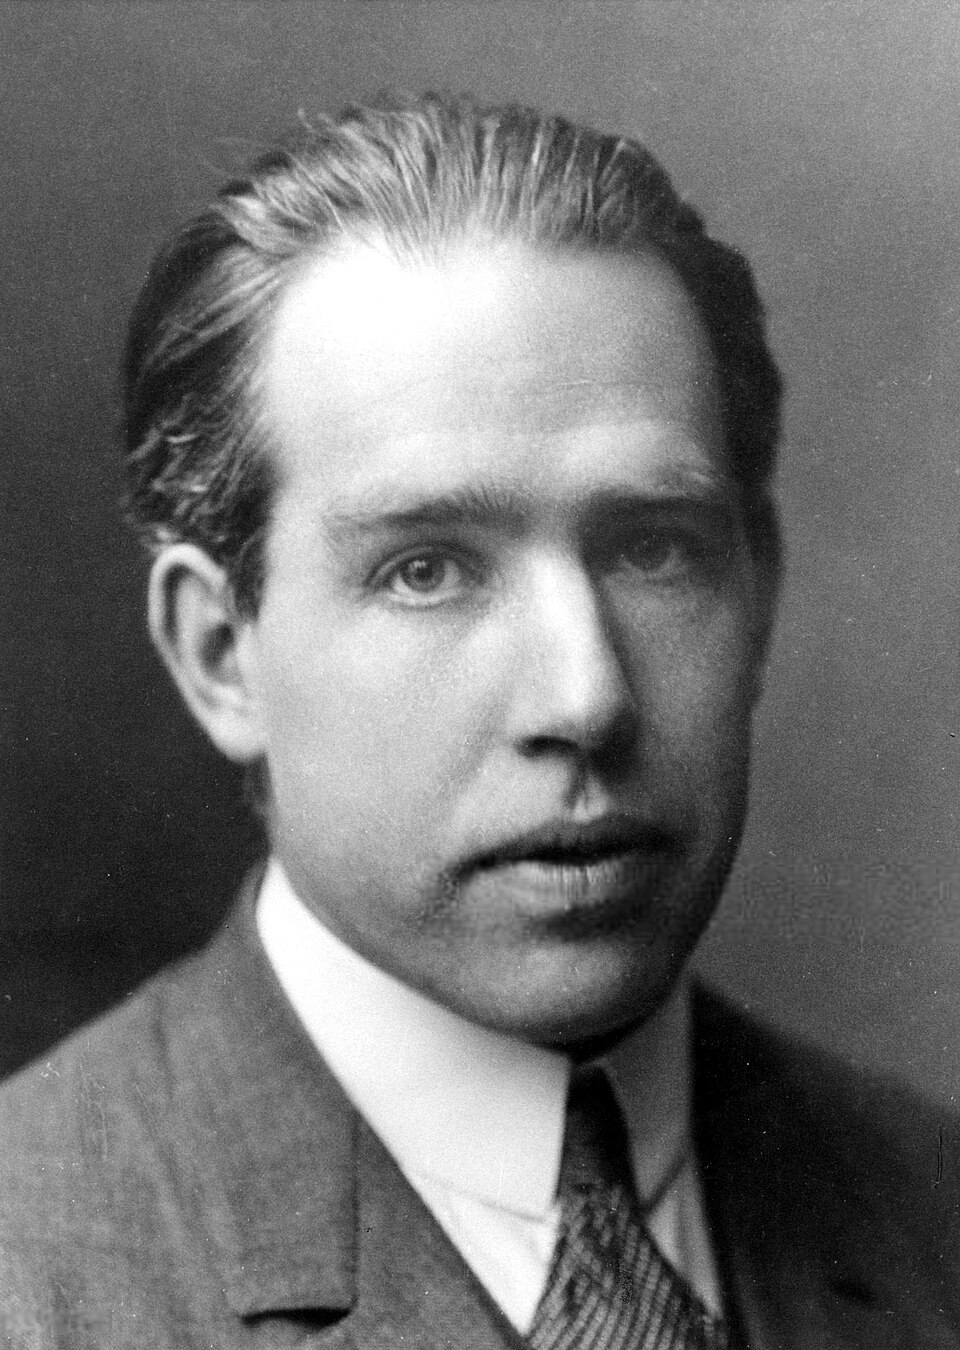
\includegraphics[width=0.26\linewidth]{images/book2/bohr.jpg}

{\small Niels Bohr (1885--1962), por volta de 1922.}
\end{omfigure}

\section{Quatro números quânticos}

Em um átomo com vários elétrons, as energias já não são dadas por uma
única fórmula, mas cada elétron continua descrito por um pequeno
conjunto de inteiros, os seus números quânticos.

\begin{definition}[Números quânticos]\label{def:b1:quantum-numbers:quantum-number}
O estado de um elétron em um átomo é identificado por quatro números:
\begin{itemize}
  \item o \emph{número quântico principal}\index{numero quantico principal@número quântico principal}
        $n = 1, 2, 3, \dots$, que fixa principalmente a energia e o tamanho;
  \item o \emph{número quântico azimutal}\index{numero quantico azimutal@número quântico azimutal}
        (ou número quântico secundário) $l = 0, 1, \dots, n-1$, que fixa
        a forma; $l = 0, 1, 2, 3$ são indicados por s, p, d, f;
  \item o \emph{número quântico magnético}\index{numero quantico magnetico@número quântico magnético}
        $m_l = -l, -l+1, \dots, l$, que fixa a orientação ($2l + 1$
        valores);
  \item o \emph{número quântico de spin}\index{numero quantico de spin@número quântico de spin}
        $m_s = +\tfrac12$ ou $-\tfrac12$, uma propriedade intrínseca do
        elétron, representada por uma seta para cima ou para baixo.
\end{itemize}
\end{definition}

\begin{definition}[Orbital atômico, camada, subcamada]\label{def:b1:quantum-numbers:orbital}
Um \emph{orbital atômico}\index{orbital atomico@orbital atômico} é o estado de um elétron
identificado pelos três números $(n, l, m_l)$; ele é representado por uma
caixa, \omorbs{}. Os orbitais de mesmo $n$ formam uma \emph{camada
eletrônica}\index{camada eletronica@camada eletrônica}; os de mesmos $n$ e $l$ formam uma
\emph{subcamada}\index{subcamada}, designada por $n$ e pela letra de $l$:
2p é a subcamada $n = 2$, $l = 1$, formada por três orbitais
($m_l = -1, 0, 1$).
\end{definition}

\begin{remark}[Formas]\label{rem:b1:quantum-numbers:shapes}
Um orbital s é esférico; um orbital p tem dois lobos ao longo de um eixo,
e os três orbitais 2p apontam ao longo de $x$, $y$ e $z$. A descrição
matemática dessas formas --- funções de onda, suas partes radial e
angular, seus nós --- pertence ao volume do 2.º ano. Neste livro, um
orbital é uma caixa que comporta no máximo dois elétrons.
\end{remark}

\begin{proposition}[Capacidade de uma subcamada e de uma camada]\label{prop:b1:quantum-numbers:capacity}
Uma \omterm{def:b1:quantum-numbers:orbital}{subcamada} de número azimutal $l$ contém $2l + 1$ orbitais e comporta
$2(2l + 1)$ elétrons: 2 em s, 6 em p, 10 em d, 14 em f. A camada $n$
contém $n^2$ orbitais e comporta $2n^2$ elétrons.
\end{proposition}

\begin{proof}
Para um $l$ dado, $m_l$ assume os $2l + 1$ valores de $-l$ a $l$, e
cada orbital comporta dois elétrons de spins opostos (\cref{prop:b1:quantum-numbers:pauli}
adiante). Para um $n$ dado, $l$ vai de $0$ a $n - 1$, de modo que o
número de orbitais é
\[
  \sum_{l=0}^{n-1} (2l+1) = 2\,\frac{(n-1)n}{2} + n = n^2 ,
\]
e o número de elétrons é $2n^2$: 2, 8, 18, 32 para $n = 1$ a 4.
\end{proof}

\begin{example}[A terceira camada]\label{ex:b1:quantum-numbers:third}
Para $n = 3$: $l = 0$ (3s, um orbital), $l = 1$ (3p, três orbitais),
$l = 2$ (3d, cinco orbitais, $m_l = -2, \dots, 2$): nove orbitais e até
18 elétrons. Um elétron em 3d tem, por exemplo, os números
quânticos $(3, 2, -1, +\tfrac12)$.
\end{example}

\section{Construção das configurações}

\begin{definition}[Configuração eletrônica]\label{def:b1:quantum-numbers:configuration}
A \emph{configuração eletrônica}\index{configuracao eletronica@configuração eletrônica} de um
átomo ou íon é a lista de suas \omterm{def:b1:quantum-numbers:orbital}{subcamadas} ocupadas, com o número de
elétrons de cada uma escrito como expoente: $1\text{s}^2 2\text{s}^2
2\text{p}^4$ para o oxigênio. Os elétrons de maior $n$, junto com os de
uma \omterm{def:b1:quantum-numbers:orbital}{subcamada} d ou f incompleta, são os \emph{elétrons de
valência}\index{eletrons de valencia@elétrons de valência}; os outros são os \emph{elétrons de
caroço}\index{eletrons de caroco@elétrons de caroço}. Uma configuração é abreviada
escrevendo-se entre colchetes a configuração do gás nobre anterior:
o oxigênio é $[\ce{He}]\,2\text{s}^2 2\text{p}^4$.
\end{definition}

Três regras fornecem a configuração do \omterm{def:b1:quantum-numbers:energy-level}{estado fundamental}.

\begin{proposition}[Princípio de exclusão de Pauli]\label{prop:b1:quantum-numbers:pauli}
Dois elétrons de um mesmo átomo nunca têm os mesmos quatro números
quânticos. Logo, um orbital comporta no máximo dois elétrons, e então
com spins opostos: \omorbs{ud}.
\end{proposition}
\admitted

\begin{proposition}[Regra de Klechkowski]\label{prop:b1:quantum-numbers:klechkowski}
No \omterm{def:b1:quantum-numbers:energy-level}{estado fundamental} de um átomo neutro, as \omterm{def:b1:quantum-numbers:orbital}{subcamadas} são preenchidas
na ordem crescente de $n + l$ e, para $n + l$ iguais, na ordem crescente
de $n$:
\[
  1\text{s},\ 2\text{s},\ 2\text{p},\ 3\text{s},\ 3\text{p},\ 4\text{s},\
  3\text{d},\ 4\text{p},\ 5\text{s},\ 4\text{d},\ 5\text{p},\ 6\text{s},\
  4\text{f},\ 5\text{d},\ 6\text{p},\ 7\text{s},\ 5\text{f},\ 6\text{d},\
  7\text{p}.
\]
\end{proposition}
\admitted

\begin{remark}[Uma regra empírica]\label{rem:b1:quantum-numbers:klech-empirical}
A regra de Klechkowski (também chamada regra de Madelung) resume
configurações observadas; não é uma lei: descreve a ordem em que as
\omterm{def:b1:quantum-numbers:orbital}{subcamadas} se preenchem à medida que a carga nuclear aumenta. Em um
átomo com vários elétrons, os elétrons se repelem, de modo que a energia
de uma \omterm{def:b1:quantum-numbers:orbital}{subcamada} depende de $l$ além de $n$: um elétron 4s, que passa
parte do tempo perto do núcleo, acaba abaixo de 3d no potássio e no cálcio.
\end{remark}

\begin{omfigure}
\begin{tikzpicture}[font=\small, x=1.25cm, y=0.72cm]
  \foreach \n in {1,...,7} {
    \foreach \l/\s in {0/s,1/p,2/d,3/f} {
      \pgfmathtruncatemacro\ok{(\l<\n) && (\n+\l<=8)}
      \ifnum\ok=1
        \node[draw=black!50, rounded corners=2pt, minimum width=0.85cm,
          minimum height=0.5cm, fill=white] (s\n\l) at (\l,-\n) {\n\s};
      \fi
    }
  }
  \begin{scope}[on background layer]
  \foreach \la/\na/\lb/\nb in {0/1/0/1, 0/2/0/2, 1/2/0/3, 1/3/0/4, 2/3/0/5,
      2/4/0/6, 3/4/0/7, 3/5/1/7} {
    \draw[-{Stealth}, omDef, thick, opacity=0.8]
      ($(\la,-\na)+(0.5,0.42)$) -- ($(\lb,-\nb)+(-0.5,-0.42)$);
  }
  \end{scope}
  \node[anchor=west, align=left, font=\small] at (4.0,-2.5) {siga cada seta,\\depois a seguinte,\\à sua direita};
\end{tikzpicture}

{\small O diagrama de Klechkowski. As \omterm{def:b1:quantum-numbers:orbital}{subcamadas} de mesmo $n + l$ ficam
em uma mesma diagonal; percorrer as diagonais em ordem fornece a ordem de
preenchimento 1s, 2s, 2p, 3s, 3p, 4s, 3d, 4p, 5s, \dots}
\end{omfigure}

\begin{proposition}[Regra de Hund]\label{prop:b1:quantum-numbers:hund}
Quando os elétrons de uma \omterm{def:b1:quantum-numbers:orbital}{subcamada} podem ser colocados em vários
orbitais de mesma energia, o \omterm{def:b1:quantum-numbers:energy-level}{estado fundamental} tem o maior número
possível de spins \emph{paralelos}: os elétrons ocupam orbitais
separados, com spin para cima, antes que algum orbital receba dois.
\end{proposition}
\admitted

\begin{definition}[Elétron desemparelhado]\label{def:b1:quantum-numbers:unpaired}
Um \emph{elétron desemparelhado}\index{eletron desemparelhado@elétron desemparelhado} é um elétron
sozinho em seu orbital. Uma espécie com elétrons desemparelhados é
atraída por um ímã (ela é paramagnética, propriedade estudada na física).
\end{definition}

\begin{method}[Escrever a configuração de um estado fundamental]\label{met:b1:quantum-numbers:configuration}
Para escrever a configuração de um átomo de número atômico $Z$:
\begin{enumerate}
  \item coloque $Z$ elétrons nas \omterm{def:b1:quantum-numbers:orbital}{subcamadas} na ordem de Klechkowski,
        completando cada \omterm{def:b1:quantum-numbers:orbital}{subcamada} (2, 6, 10, 14) antes da seguinte;
  \item escreva o resultado na ordem crescente de $n$ (agrupando 3d
        com $n = 3$) e abrevie com o cerne do gás nobre
        anterior;
  \item para a última \omterm{def:b1:quantum-numbers:orbital}{subcamada}, incompleta, desenhe as caixas e
        aplique a regra de Hund para contar os \omterm{def:b1:quantum-numbers:unpaired}{elétrons desemparelhados}.
\end{enumerate}
\end{method}

\begin{example}[Carbono, nitrogênio, oxigênio, ferro]\label{ex:b1:quantum-numbers:examples}
O método fornece, para quatro átomos:
\begin{center}
\begin{tabular}{lllc}
\hline
átomo & configuração & última \omterm{def:b1:quantum-numbers:orbital}{subcamada} & desemparelhados \\
\hline
\ce{C} ($Z = 6$) & $[\ce{He}]\,2\text{s}^2 2\text{p}^2$ & 2p: \omorbs{u,u,} & 2 \\
\ce{N} ($Z = 7$) & $[\ce{He}]\,2\text{s}^2 2\text{p}^3$ & 2p: \omorbs{u,u,u} & 3 \\
\ce{O} ($Z = 8$) & $[\ce{He}]\,2\text{s}^2 2\text{p}^4$ & 2p: \omorbs{ud,u,u} & 2 \\
\ce{Fe} ($Z = 26$) & $[\ce{Ar}]\,3\text{d}^6 4\text{s}^2$ & 3d: \omorbs{ud,u,u,u,u} & 4 \\
\hline
\end{tabular}
\end{center}
Para o ferro, a ordem de Klechkowski preenche 4s ($Z = 19, 20$) antes de 3d
($Z = 21$ a 30); a configuração é escrita com 3d primeiro.
% ledger: gs:Fe
\end{example}

\begin{omfigure}
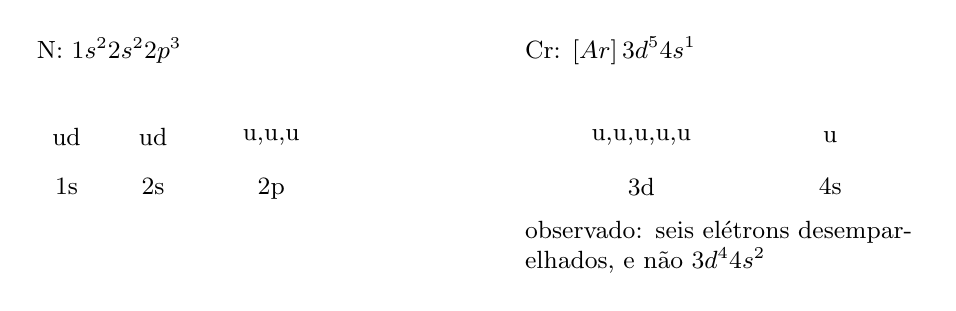
\begin{tikzpicture}[font=\small]
  \begin{scope}
    \node[anchor=west] at (0,2.4) {\ce{N}: $1\text{s}^2 2\text{s}^2 2\text{p}^3$};
    \node at (0.5,1.3) {\omorbs{ud}}; \node[below] at (0.5,0.9) {1s};
    \node at (1.6,1.3) {\omorbs{ud}}; \node[below] at (1.6,0.9) {2s};
    \node at (3.1,1.3) {\omorbs{u,u,u}}; \node[below] at (3.1,0.9) {2p};
  \end{scope}
  \begin{scope}[xshift=6.2cm]
    \node[anchor=west] at (0,2.4) {\ce{Cr}: $[\ce{Ar}]\,3\text{d}^5 4\text{s}^1$};
    \node at (1.6,1.3) {\omorbs{u,u,u,u,u}}; \node[below] at (1.6,0.9) {3d};
    \node at (4.0,1.3) {\omorbs{u}}; \node[below] at (4.0,0.9) {4s};
    \node[anchor=west, text width=5.0cm] at (0,-0.1) {observado: seis elétrons desemparelhados, e não $3\text{d}^4 4\text{s}^2$};
  \end{scope}
\end{tikzpicture}

{\small Caixas quânticas. Cada caixa é um orbital; uma seta é um elétron
e seu spin. O nitrogênio segue a regra de Hund; o cromo é uma das
exceções da \cref{prop:b1:quantum-numbers:exceptions}.}
\end{omfigure}

\section{Íons, exceções e a forma da tabela}

\begin{proposition}[Configurações dos íons]\label{prop:b1:quantum-numbers:ions}
Um ânion monoatômico tem a configuração do átomo com os elétrons
adicionais colocados nos lugares seguintes da ordem de Klechkowski; um
cátion de um elemento representativo perde os elétrons de maior $n$. Um
cátion de metal de transição perde seus elétrons $n$s \emph{antes} dos
elétrons $(n-1)$d: \ce{Fe^{2+}} é $[\ce{Ar}]\,3\text{d}^6$ e
\ce{Fe^{3+}} é $[\ce{Ar}]\,3\text{d}^5$, e não $[\ce{Ar}]\,3\text{d}^4
4\text{s}^2$.
% ledger: gs:Fe2+, gs:Fe3+
\end{proposition}
\admitted

\begin{remark}[Ordem de preenchimento não é ordem de remoção]\label{rem:b1:quantum-numbers:order}
4s se preenche antes de 3d no potássio e no cálcio, e no entanto é
esvaziada primeiro nos íons dos metais de transição. Não há contradição:
a ordem das energias das \omterm{def:b1:quantum-numbers:orbital}{subcamadas} muda com a carga nuclear e com o
número de elétrons, e em um átomo ou íon de metal de transição a
\omterm{def:b1:quantum-numbers:orbital}{subcamada} 3d fica abaixo de 4s. A regra de Klechkowski descreve apenas
átomos neutros.
\end{remark}

\begin{proposition}[Duas exceções na primeira série de transição]\label{prop:b1:quantum-numbers:exceptions}
As configurações observadas do \omterm{def:b1:quantum-numbers:energy-level}{estado fundamental} do cromo e do cobre são
\[
  \ce{Cr}: [\ce{Ar}]\,3\text{d}^5 4\text{s}^1, \qquad
  \ce{Cu}: [\ce{Ar}]\,3\text{d}^{10} 4\text{s}^1 ,
\]
em vez de $3\text{d}^4 4\text{s}^2$ e $3\text{d}^9 4\text{s}^2$,
previstas pela regra de Klechkowski: uma \omterm{def:b1:quantum-numbers:orbital}{subcamada} d semipreenchida ou
completa é especialmente estável, e os níveis 4s e 3d são próximos.
% ledger: gs:Cr, gs:Cu
\end{proposition}

\begin{example}[O cobre e seus íons]\label{ex:b1:quantum-numbers:copper}
\ce{Cu} é $[\ce{Ar}]\,3\text{d}^{10} 4\text{s}^1$; \ce{Cu+} é
$[\ce{Ar}]\,3\text{d}^{10}$, sem \omterm{def:b1:quantum-numbers:unpaired}{elétron desemparelhado}; \ce{Cu^{2+}} é
$[\ce{Ar}]\,3\text{d}^9$, com um. \ce{Zn^{2+}}, $[\ce{Ar}]\,3\text{d}^{10}$,
não tem nenhum.
% ledger: gs:Cu+, gs:Cu2+, gs:Zn2+
\end{example}

\begin{proposition}[Configurações e a tabela periódica]\label{prop:b1:quantum-numbers:table}
O período $n$ da tabela periódica começa com o preenchimento de $n$s e
termina com o preenchimento de $n$p. As \omterm{def:b1:quantum-numbers:orbital}{subcamadas} preenchidas entre eles
são, pela regra de Klechkowski, $(n-2)$f e $(n-1)$d. Assim, os períodos
contêm $2, 8, 8, 18, 18, 32, 32$ elementos, e os gases nobres têm $Z = 2, 10,
18, 36, 54, 86, 118$.
\end{proposition}

\begin{proof}
Os períodos 1 a 3 contêm apenas $n$s (e $n$p para $n \ge 2$): $2$, depois
$2 + 6 = 8$ duas vezes. Nos períodos 4 e 5, acrescenta-se $(n-1)$d: $2 + 10 + 6 =
18$. Nos períodos 6 e 7, também $(n-2)$f: $2 + 14 + 10 + 6 = 32$. Os
gases nobres fecham cada período: $2$, $2 + 8 = 10$, $18$, $18 + 18 = 36$,
$54$, $54 + 32 = 86$, $118$.
\end{proof}

\begin{omfigure}
\omperiodictable[colour=blocks, legend]

{\small A tabela periódica colorida segundo a última \omterm{def:b1:quantum-numbers:orbital}{subcamada} em
preenchimento: os blocos s, p, d e f. A largura de cada bloco é a
capacidade de sua \omterm{def:b1:quantum-numbers:orbital}{subcamada}, 2, 6, 10 e 14.}
\end{omfigure}

\section{Exercícios}

\begin{exercise}[$\star$]\label{exo:b1:quantum-numbers:1}
Quais destes conjuntos $(n, l, m_l, m_s)$ podem descrever um elétron em
um átomo? Justifique cada recusa.
(a) $(2, 2, 0, +\tfrac12)$; (b) $(3, 1, -1, -\tfrac12)$;
(c) $(1, 0, 0, 0)$; (d) $(4, 3, -3, +\tfrac12)$; (e) $(3, 0, 1, -\tfrac12)$.
\end{exercise}

\begin{exercise}[$\star$]\label{exo:b1:quantum-numbers:2}
Quantos orbitais, e no máximo quantos elétrons, há nas \omterm{def:b1:quantum-numbers:orbital}{subcamadas} 3d, 4f
e 5p, e na camada $n = 2$?
\end{exercise}

\begin{exercise}[$\star$]\label{exo:b1:quantum-numbers:3}
Escreva as configurações do \omterm{def:b1:quantum-numbers:energy-level}{estado fundamental} de \ce{O}, \ce{P}, \ce{K}, \ce{Ca}
e \ce{Br} ($Z = 8, 15, 19, 20, 35$), por extenso e abreviadas, e dê o
número de \omterm{def:b1:quantum-numbers:configuration}{elétrons de valência} de cada um.
\end{exercise}

\begin{exercise}[$\star$]\label{exo:b1:quantum-numbers:4}
Desenhe as caixas quânticas das \omterm{def:b1:quantum-numbers:orbital}{subcamadas} de valência do nitrogênio, do
enxofre e do cloro, e conte seus \omterm{def:b1:quantum-numbers:unpaired}{elétrons desemparelhados}.
\end{exercise}

\begin{exercise}[$\star\star$]\label{exo:b1:quantum-numbers:5}
Dê as configurações de \ce{Na+}, \ce{Mg^{2+}}, \ce{Al^{3+}}, \ce{F-},
\ce{O^{2-}}, \ce{Cl-}, \ce{S^{2-}} e \ce{Ca^{2+}}. Com qual gás nobre
cada um é isoeletrônico?
\end{exercise}

\begin{exercise}[$\star\star$]\label{exo:b1:quantum-numbers:6}
Escreva as configurações de \ce{Ti^{2+}}, \ce{Mn^{2+}}, \ce{Co^{2+}},
\ce{Ni^{2+}} e \ce{Zn^{2+}} ($Z = 22, 25, 27, 28, 30$) e dê o
número de \omterm{def:b1:quantum-numbers:unpaired}{elétrons desemparelhados} de cada um.
\end{exercise}

\begin{exercise}[$\star\star$]\label{exo:b1:quantum-numbers:7}
Calcule a energia e o comprimento de onda do fóton emitido na
transição $4 \to 3$ do hidrogênio. Em que região do espectro ele está?
Considere $E_R = \qty{13.6}{eV}$ e $hc = \qty{1240}{eV.nm}$.
\end{exercise}

\begin{exercise}[$\star\star$]\label{exo:b1:quantum-numbers:8}
Identifique os elementos cujas configurações do \omterm{def:b1:quantum-numbers:energy-level}{estado fundamental} terminam em
(a) $3\text{s}^2 3\text{p}^4$; (b) $4\text{s}^2 3\text{d}^{10} 4\text{p}^5$;
(c) $5\text{s}^1$; (d) $4\text{s}^2 3\text{d}^3$. Dê os quatro números
quânticos de um elétron da última \omterm{def:b1:quantum-numbers:orbital}{subcamada} de (a).
\end{exercise}

\begin{exercise}[$\star\star$]\label{exo:b1:quantum-numbers:9}
Usando a regra de Klechkowski, explique por que o décimo nono elétron do
potássio vai para 4s e não para 3d, e por que o período 3 contém 8
elementos e não 18.
\end{exercise}

\begin{exercise}[$\star\star\star$]\label{exo:b1:quantum-numbers:10}
Um íon com um único elétron e um núcleo de carga $Ze$ tem níveis
$E_n = -Z^2 E_R/n^2$ (admitido). Para \ce{He+} ($Z = 2$), calcule a
energia de ionização e o comprimento de onda da transição $2 \to 1$.
Compare com o hidrogênio.
\end{exercise}

\begin{exercise}[$\star\star\star$]\label{exo:b1:quantum-numbers:11}
Diga se cada configuração é um \omterm{def:b1:quantum-numbers:energy-level}{estado fundamental}, um \omterm{def:b1:quantum-numbers:energy-level}{estado excitado} ou
impossível, e por quê: (a) $1\text{s}^2 2\text{s}^1 2\text{p}^1$;
(b) $1\text{s}^2 2\text{s}^2 2\text{p}^7$; (c) $1\text{s}^2 2\text{p}^2$;
(d) $[\ce{Ne}]\,3\text{s}^2 3\text{p}^3$; (e) $1\text{s}^3$.
\end{exercise}

\begin{exercise}[$\star\star\star$]\label{exo:b1:quantum-numbers:12}
Os sais de ferro(III) são atraídos por um ímã com mais força que os sais
de ferro(II), e os sais de zinco não são atraídos. Ordene \ce{Fe^{2+}}, \ce{Fe^{3+}},
\ce{Mn^{2+}}, \ce{Cu^{2+}} e \ce{Zn^{2+}} pelo número de \omterm{def:b1:quantum-numbers:unpaired}{elétrons
desemparelhados} e explique a observação, supondo que a atração cresce
com esse número.
\end{exercise}

\section{Problema: As raias de uma lâmpada, e um mundo com três spins}

\begin{problem}[{Problema de fim de semana --- das quatro raias de uma lâmpada de
hidrogênio ao comprimento dos períodos, e como seria a tabela se um
elétron tivesse três estados de spin}]
\label{pb:b1:quantum-numbers:1}
Considere $E_R = \qty{13.6}{eV}$ e $hc = \qty{1240}{eV.nm}$ em todo o problema.
A faixa visível vai de cerca de 400 a \qty{700}{nm}.

\medskip
\noindent\textbf{Parte I --- A lâmpada de hidrogênio.}
\begin{enumerate}
  \item Calcule as energias $E_1$ a $E_4$ do átomo de hidrogênio.
  \item Calcule a energia e o comprimento de onda do fóton emitido na
        transição $3 \to 2$. Qual é a sua cor?
  \item Calcule os comprimentos de onda das transições $4 \to 2$, $5 \to 2$
        e $6 \to 2$.
  \item Por que uma lâmpada de hidrogênio mostra exatamente quatro raias
        visíveis? Calcule o comprimento de onda de $7 \to 2$ para apoiar a resposta.
  \item Calcule o limite da série de Balmer.
  \item Calcule o comprimento de onda da primeira raia de Lyman, $2 \to 1$.
        Por que ela não pode ser vista?
  \item Qual é o maior comprimento de onda de um fóton capaz de ionizar
        um átomo de hidrogênio em seu \omterm{def:b1:quantum-numbers:energy-level}{estado fundamental}?
\end{enumerate}

\medskip
\noindent\textbf{Parte II --- Contagem de estados.}
\begin{enumerate}[resume]
  \item Liste os valores de $l$ e $m_l$ para $n = 3$; quantos orbitais
        a camada contém?
  \item Mostre que a camada $n$ comporta $2n^2$ elétrons; aplique a $n = 4$.
  \item Escreva a ordem de Klechkowski até 7p.
  \item Deduza os comprimentos dos sete períodos.
  \item Explique por que a \omterm{def:b1:quantum-numbers:orbital}{subcamada} 3d não aparece no período 3.
  \item Deduza os números atômicos dos gases nobres.
\end{enumerate}

\medskip
\noindent\textbf{Parte III --- Os metais de transição.}
\begin{enumerate}[resume]
  \item Escreva a configuração do ferro ($Z = 26$) e desenhe suas caixas
        3d. Quantos \omterm{def:b1:quantum-numbers:unpaired}{elétrons desemparelhados}?
  \item Mesmas perguntas para \ce{Fe^{2+}} e \ce{Fe^{3+}}. Qual dos dois
        tem uma \omterm{def:b1:quantum-numbers:orbital}{subcamada} semipreenchida?
  \item A configuração observada do cromo é $[\ce{Ar}]\,3\text{d}^5
        4\text{s}^1$. Compare com a previsão e conte os \omterm{def:b1:quantum-numbers:unpaired}{elétrons
        desemparelhados} em cada caso.
  \item Dê as configurações de \ce{Cu}, \ce{Cu+} e \ce{Cu^{2+}}.
  \item Qual de \ce{Cu+} e \ce{Cu^{2+}} tem \omterm{def:b1:quantum-numbers:unpaired}{elétrons desemparelhados}?
  \item Entre \ce{Sc^{3+}}, \ce{Ti^{3+}}, \ce{Mn^{2+}} ($Z = 21, 22, 25$),
        qual tem mais \omterm{def:b1:quantum-numbers:unpaired}{elétrons desemparelhados}?
\end{enumerate}

\medskip
\noindent\textbf{Parte IV --- Um mundo com três spins.}
Imagine um universo em que $n$, $l$ e $m_l$ obedecem às mesmas regras
que no nosso, a ordem de Klechkowski não muda, o princípio de exclusão
vale, mas o número de spin $m_s$ pode assumir três valores.
\begin{enumerate}[resume]
  \item Quantos elétrons um orbital pode comportar? Uma \omterm{def:b1:quantum-numbers:orbital}{subcamada} de
        número $l$? Uma camada $n$?
  \item Dê as capacidades de 1s, 2s, 2p, 3s e 3p.
  \item Um gás nobre fecha um período com uma \omterm{def:b1:quantum-numbers:orbital}{subcamada} p completa (ou 1s,
        no caso do primeiro). Qual é o número atômico do primeiro gás nobre?
  \item Qual número atômico se comportaria como um metal alcalino, com
        um único elétron além do primeiro gás nobre?
  \item Quantos elementos teria o segundo período?
  \item Calcule o número atômico do segundo gás nobre desse mundo.
\end{enumerate}
\end{problem}
